\documentclass[11pt,a4paper]{book}
\usepackage[brazilian]{babel}
\usepackage[utf8]{inputenc}
\usepackage[T1]{fontenc}
\usepackage[inline]{enumitem}
\usepackage{xcolor}
\usepackage{listings}
\usepackage{graphicx}
\usepackage{multicol}
\usepackage{amsmath}
\usepackage{amssymb}

\definecolor{mGreen}{rgb}{0,0.6,0}
\definecolor{mGray}{rgb}{0.5,0.5,0.5}
\definecolor{mPurple}{rgb}{0.58,0,0.82}
\definecolor{backgroundColour}{rgb}{0.95,0.95,0.92}

\lstdefinestyle{CStyle}{
    backgroundcolor=\color{backgroundColour},   
    commentstyle=\color{mGreen},
    keywordstyle=\textbf{\color{black}},
    numberstyle=\tiny\color{mGray},
    stringstyle=\color{mPurple},
    basicstyle=\footnotesize,
    breakatwhitespace=false,         
    breaklines=true,                 
    captionpos=b,                    
    keepspaces=true,                 
    numbers=left,                    
    numbersep=5pt,                  
    showspaces=false,                
    showstringspaces=false,
    showtabs=false,                  
    tabsize=2,
    frame=single,
    escapeinside={(*}{*)},
    language=C
}

\makeatletter
% This command ignores the optional argument for itemize and enumerate lists
\newcommand{\inlineitem}[1][]{%
\ifnum\enit@type=\tw@
    {\descriptionlabel{#1}}
  \hspace{\labelsep}
\else
  \ifnum\enit@type=\z@
       \refstepcounter{\@listctr}\fi
    \quad\@itemlabel\hspace{\labelsep}
\fi}
\makeatother

\newcommand{\onestaritem}{\refstepcounter{enumi}\item[$*$\theenumi.]}
\newcommand{\twostaritem}{\refstepcounter{enumi}\item[$**$\theenumi.]}
\DeclareMathOperator*{\maxi}{max}

\title{Lista 10: Fundamentos Estatísticos para Ciência dos Dados}
\author{Ricardo Pagoto Marinho}

\begin{document}
\maketitle
	\begin{enumerate}
		\item
		\begin{enumerate}[label=\alph*)]
			\item
			Seja B uma matriz definida positiva \textit{pxp} com autovetores $\lambda_1 \geq\lambda_2\geq \ldots\lambda_p > 0$ e autovetores associados $v_1, v_2,\ldots, v_p$ de comprimento 1.
			Então
			\begin{eqnarray*}
				\maxi_{\mathbf{x\neq 0}} \frac{x'Bx}{x'x}=\lambda_1
			\end{eqnarray*}
			
			quando $x=v_1$.
			
			Prova:
			
			Seja P uma matriz ortogonal \textit{pxp} na qual suas colunas sejam os autovetores $v_1, v_2,\ldots, v_p$ e $\Lambda$ a matriz diagonal com os autovalores $\lambda_1, \lambda_2, \ldots \lambda_p$ formando a diagonal principal.
			Seja $B^{\frac{1}{2}}=P\Lambda P'$ e y e x, vetores \textit{px1} tais que $y=P'x$.
			
			Consequentemente, $x\neq 0$ implica em $y\neq 0$.
			Assim:
			
			\begin{eqnarray*}
				\frac{x'Bx}{x'x}=\frac{x'B^{\frac{1}{2}}B^{\frac{1}{2}}x}{x'P'Px}=\\
				\frac{x'P\Lambda^{\frac{1}{2}} P' P\Lambda^{\frac{1}{2}}P'x}{y'y}=\frac{y'\Lambda y}{y'y}=\\
				\frac{\sum_{i=1}^{p}\lambda_i y_i^2}{\sum_{i=1}^{p}y_i^2}\leq \lambda_1\frac{\sum_{i=1}^{p}y_i^2}{\sum_{i=1}^{p}y_i^2}=\lambda_1
			\end{eqnarray*}
			
			Fazendo $x=v_1$, temos:
			
			\begin{eqnarray*}
				y=P'v_1=
				\left[\begin{tabular}{c}
				1\\
				0\\
				\vdots\\
				0
				\end{tabular}
				\right]
			\end{eqnarray*}
			
			já que
			\begin{eqnarray*}
				e_k e_1=\left\lbrace
				\begin{tabular}{c l}
				1, & k=1\\
				0, & $k\neq 1$
				\end{tabular}
				\right.
			\end{eqnarray*}
			
			Para esta escolha de x, temos $\frac{y'\Lambda y}{y'y}=\frac{\lambda_1}{1}=\lambda_1$, ou ainda:
			
			\begin{eqnarray*}
				\frac{v_1'Bv_1}{v_1'v_1}=v_1'Bv_1=\lambda_1
			\end{eqnarray*}
			
			\item 
			Seja $\sum$ a matriz de covariância associada ao vetor aleatório $X=\left[ X_1,X_2,\ldots,X_p\right]$, com auto valores $\lambda_1 \geq\lambda_2\geq \ldots\lambda_p > 0$ e autovetores associados $v_1, v_2,\ldots, v_p$ de comprimento 1.
			Então, a combinação linear $Y=l'Y=l_1X_1+\ldots +l_pX_p$ de comprimento ||l||=1 e que maximiza $\mathbb{V}(Y)$ é obtida ao tomarmos l igual ao primeiro autovetor.
			Neste caso, $Y=v_1'X$ e a variância desta variável atinge $\mathbb{V}(Y)=\lambda_1$.
			
			Prova:
			
			Da prova do item anterior, sabemos que
			
			\begin{eqnarray*}
				\maxi_{\mathbf{a\neq 0}} \frac{a'\sum a}{a'a}=\lambda_1 & (obtida~quando~a=v_1)
			\end{eqnarray*}
			
			Porém, $v_1'v_1=1$, já que os autovetores são normalizados.
			Assim:
			
			\begin{eqnarray*}
				\maxi_{\mathbf{a\neq 0}} \frac{a'\sum a}{a'a}=\lambda_1=\frac{v_1'\sum v_1}{v_1'v_1}=v_1'\sum v_1=Var(Y_1)
			\end{eqnarray*}
			
			Similarmente
			
			\begin{eqnarray*}
				\maxi_{\mathbf{a\perp v_1,v_2,\ldots,v_k}} \frac{a'\sum a}{a'a}=\lambda_{k+1} & k=1,2,\ldots,p-1
			\end{eqnarray*}
			
			Escolhendo $a=v_{k+1}$, com $v_{k+1}'v_i=0$, para $i=1,2,\ldots,k$ e $k=1,2,\ldots,p-1$,
			
			\begin{eqnarray*}
				\frac{v_{k+1}'\sum v_{k+1}}{v_{k_1}'v_{k+1}}=v_{k+1}'\sum v_{k+1}=Var(Y_{k+1})
			\end{eqnarray*}
			
			Porém,
			
			\begin{eqnarray*}
				\frac{v_{k+1}'\sum v_{k+1}}{v_{k_1}'v_{k+1}}=\lambda_{k+1}\\
				v_{k+1}'\sum v_{k+1}=\lambda_{k+1}v_{k_1}'v_{k+1}=\lambda_{k+1}
			\end{eqnarray*}
			
			Portanto, $Var(Y_{k+1})=\lambda_{k+1}$.
			Agora, mostrarei que $v_j \perp V_k$ (ou seja, $v_iv_k=0, i\neq k$) faz com que $Cov(Y_i,Y_k)=0$.
			Os autovetores de $\sum$ são ortogonais caso todos os autovalores $\lambda_1, \lambda_2, \ldots \lambda_p$ sejam distintos.
			Se os autovalores não são todos distintos, os autovetores correspondentes a autovalores iguais, podem ser escolhidos como ortogonais.
			Portanto, para cada dupla de autovetores $v_i$ e $v_k$, $v_i'v_k=0, i\neq k$.
			Como $\sum v_k=\lambda_k v_k$, multiplicando ambos os lados por $v_i'$, temos:
			
			\begin{eqnarray*}
				Cov(Y_i,Y_k)=v_i'\sum v_k=v_i'\lambda_k v_k=\lambda_k v_i'v_k=0
			\end{eqnarray*}
			
			para qualquer $i\neq k$.
		\end{enumerate}
		
		\item
		
		O problema 8.11 do livro pede para considerar a tabela 8.5 (que está disponível online) porém multiplicando a última coluna (valor médio de casas) por 10, já que pede que o valor seja em dezenas de milhares, ao invés de centenas de milhares.
			\begin{enumerate}[label=\alph*)]
				\item O seguinte código foi utilizado para construir a matriz de covariância da amostra, considerando que os dados estão na pasta "Wichern\_data", dentro do diretório corrente:
				\begin{lstlisting}
dados<-read.csv("Wichern_data\T8-5.DAT",sep = "",header = F)
dados[,5]=dados[,5]*10
s=round(cov(dados),3)
				\end{lstlisting}
				\begin{eqnarray*}
					s=\left[
					\begin{tabular}{c c c c c}
					3.397 & -1.102 & 4.306 & -2.078 & 0.272\\
					-1.102 & 9.673 & -1.513 & 10.953 & 12.031\\
					4.306 & -1.513 & 55.626 & -28.937 & -0.436\\
					-2.078 & 10.953 & -28.937 & 89.067 & 9.573\\
					0.272 & 12.031 & -0.436 & 9.573 & 31.863
					\end{tabular}
					\right]
				\end{eqnarray*}
				Na segunda linha do código foi feita a adequação que o problema pediu.
				
				Se compararmos a matriz de covariância 's' encontrada pelo código a partir da modificação proposta com a matriz dos dados originais
				\begin{eqnarray*}
					s\_orig=\left[
					\begin{tabular}{c c c c c}
					3.397 & -1.102 & 4.306 & -2.078 & 0.027\\
					-1.102 & 9.673 & -1.513 & 10.953 & 1.203\\
					4.306 & -1.513 & 55.626 & -28.937 & -0.044\\
					-2.078 & 10.953 & -28.937 & 89.067 & 0.957\\
					0.027 & 1.203 & -0.044 & 0.957 & 0.319
					\end{tabular}
					\right]
				\end{eqnarray*}
				
				podemos observar que os elementos da última linha e da última coluna estão multiplicados por 10 e o último elemento por 100.
				Isso ocorre pelo fato de que na construção da matriz, os valores são multiplicados.
				Como a última linha e coluna são relativas à variável multiplicada por 10, seus valores na matriz de covariância também são.
				E como o último elemento da matriz é relativo a multiplicação dos valores da última variável com eles mesmos, a multiplicação fica por 100 (10x10).
				
				\item
				Utilizando as funções $eigen()$ e $prcomp()$ de R, cheguei aos seguintes resultados:
				
				\begin{itemize}
					\item Pares de autovalores-autovetores:
					\begin{eqnarray*}
						\lambda_1 = 108.27 & v_1=\left\lbrace 0.04,-0.12,0.48,-0.86,-0.13 \right\rbrace\\
						\lambda_2 = 43.14 & v_2=\left\lbrace -0.06,-0.25,-0.76, -0.32,-0.51 \right\rbrace\\
						\lambda_3 = 31.27 & v_3=\left\lbrace -0.04,0.26,-0.43,-0.39,0.77 \right\rbrace\\
						\lambda_4 = 4.60 & v_4=\left\lbrace 0.56,-0.77,-0.03,0.07,0.31 \right\rbrace\\
						\lambda_5 = 2.35 & v_5=\left\lbrace 0.83,0.52,-0.08,-0.05,-0.20 \right\rbrace\\
					\end{eqnarray*}
					
					\item Primeiros dois elementos da pca:
					
					\begin{eqnarray*}
						Y_1=&-0.50X_1+0.08X_2\\
						Y_2=&0.49X_1+0.29X_2\\
						Y_3=&-0.46X_1+0.30X_2\\
						Y_4=&0.43X_1-0.50X_2\\
						Y_5=&0.34X_1+0.75X_2
					\end{eqnarray*}
				\end{itemize}
				\item
				Para saber a proporção da variância explicada pelos dois primeiros PCAs, fazemos
					
				\begin{eqnarray*}
					\frac{\lambda_1+\lambda_2}{\lambda_1+\lambda_2+\lambda_3+\lambda_4+\lambda_5}
				\end{eqnarray*}
				
				Desta forma, o seguinte código foi utilizado:
				
				\begin{lstlisting}
ei_s=eigen(s)
round((ei_s$values[1]+ei_s$values[2])/sum(ei_s$values),2)
[1] 0.8
				\end{lstlisting}
				
				Ou seja, a proporção da variância explicada pelos dois primeiros PCAs é de 80\%.
				Essa proporção, comparada à do problema original é menor, já que lá, ela era de 92.8\%.,
				
				Comparando as matrizes de correlação do problema original e do modificado olhando os valores absolutos, percebe-se que, no geral, as correlações entre as outras variáveis aumentaram, com algumas diminuindo um pouco.
				Porém, a correlação da última variável em relação a todas, diminuiu.
				
				\begin{eqnarray*}
					s\_orig=\left[
					\begin{tabular}{c c c c c}
					1.000 & -0.906 &  0.838 & -0.786 & -0.898\\
					-0.906 &  1.000 & -0.722  & 0.804   &0.971\\
					0.838 & -0.722  & 1.000 & -0.845 & -0.673\\
					-0.786  & 0.804 & -0.845 &  1.000  & 0.657\\
					-0.898  & 0.971 & -0.673  & 0.657  & 1.000
					\end{tabular}
					\right]\\ s=\left[
					\begin{tabular}{c c c c c}
					1.000 &  -0.922 &   0.84 & 0 -0.818 &  -0.525\\
					-0.922  &  1.000 &  -0.725  &  0.650  &  0.809\\
					0.840 &  -0.725  &  1.000 &  -0.863  & -0.399\\
					-0.818  &  0.650 &  -0.863  &  1.000 &  0.201\\
					-0.525  &  0.809 &  -0.399 &   0.201  &  1.000
					\end{tabular}
					\right]
				\end{eqnarray*}	
				
				Essas observações nos mostram que a organização do problema influencia na forma com que os dados se relacionam, já que, apesar de multiplicarmos uma variável por 10, a proporção dos PCAs e sua correlação diminuíram.
			\end{enumerate}
			
			\item
			
			Dada a matriz de covariância
			
			\begin{eqnarray*}
				\sum=\left[
				\begin{tabular}{c c c }
				1.24 & 0.48 & 0.16\\
				0.48 & 0.86 & 0.12\\
				0.16 & 0.12 & 0.14
				\end{tabular}
				\right]
			\end{eqnarray*}
			
			do vetor aleatório $X=(X_1,X_2,X_3)'$, sabe-se que:
			
			\begin{eqnarray*}
				\sum = LL' + \Psi
			\end{eqnarray*}
			
			sendo que L é obtida a partir da matriz de cargas dada na expressão:
			
			\begin{eqnarray*}
				\left[
				\begin{tabular}{c}
				$X_1$\\
				$X_2$\\
				$X_3$
				\end{tabular}
				\right]=&\left[
				\begin{tabular}{c}
				1.00\\
				0.00\\
				-1.00
				\end{tabular}
				\right]+\left[
				\begin{tabular}{c}
				0.8\\
				0.6\\
				0.2
				\end{tabular}
				\right]F+\left[
				\begin{tabular}{c}
				$\xi_1$\\
				$\xi_2$\\
				$\xi_3$
				\end{tabular}
				\right]
			\end{eqnarray*}
			
			Ou seja,
			
			\begin{eqnarray*}
				L=\left[
				\begin{tabular}{c}
				0.8\\
				0.6\\
				0.2
				\end{tabular}
				\right]
			\end{eqnarray*}
			
			A matriz $\Psi$ é a matriz diagonal de covariância da matriz coluna $\xi_i$.
			
			Rearranjando a equação, podemos dizer que
			
			\begin{eqnarray*}
				\Psi= \sum - LL'
			\end{eqnarray*}
			
			Desta forma, utilizei o seguinte código para calcular $\Psi$:
			
			\begin{lstlisting}
sig=matrix(c(1.24,0.48,0.16,0.48,0.86,0.12,0.16,0.12,0.14),ncol = 3)
L=matrix(c(0.8,0.6,0.2),ncol = 1)
psi=round(sig-L%*%t(L),3)
			\end{lstlisting}
			
			Logo,
			
			\begin{eqnarray*}
				\Psi= \left[
				\begin{tabular}{c c c}
				0.6 & 0.0 & 0.0\\
				0.0 & 0.5 & 0.0\\\
				0.0 & 0.0 & 0.1
				\end{tabular}
				\right]
			\end{eqnarray*}
			
			Assim, a matriz de covariância $\sum$ do vetor aleatório $X=(X_1,X_2,X_3)'$ pode ser obtida pela expressão
			
			\begin{eqnarray*}
				\left[
				\begin{tabular}{c}
				$X_1$\\
				$X_2$\\
				$X_3$
				\end{tabular}
				\right]=&\left[
				\begin{tabular}{c}
				1.00\\
				0.00\\
				-1.00
				\end{tabular}
				\right]+\left[
				\begin{tabular}{c}
				0.8\\
				0.6\\
				0.2
				\end{tabular}
				\right]F+\left[
				\begin{tabular}{c}
				$\xi_1$\\
				$\xi_2$\\
				$\xi_3$
				\end{tabular}
				\right]
			\end{eqnarray*}
			 
			 Onde que a matriz $\Psi$ é a matriz diagonal de covariância da matriz coluna $\xi_i$.
			 
			 \item
			 	\begin{itemize}
			 	
			 	Primeiro devemos achar os autovetores da matriz de correlação X.
				Para isso, fiz as seguintes operações:
					\item
				\begin{lstlisting}
c=cor(wine[,2:14])
round(eigen(c)$vec[,1:2],2)
       [,1]  [,2]
 [1,] -0.14 -0.48
 [2,]  0.25 -0.22
 [3,]  0.00 -0.32
 [4,]  0.24  0.01
 [5,] -0.14 -0.30
 [6,] -0.39 -0.07
 [7,] -0.42  0.00
 [8,]  0.30 -0.03
 [9,] -0.31 -0.04
[10,]  0.09 -0.53
[11,] -0.30  0.28
[12,] -0.38  0.16
[13,] -0.29 -0.36
				\end{lstlisting}
				Dessa forma, temos os dois primeiros autovetores.
				Logo, os valores (??) da lista são:
				\begin{eqnarray*}
					\begin{tabular}{p{13cm}}
					$Y_{i1}=-0.14Z_{i1}+0.25Z_{i2}+0.00Z_{i3}+0.24Z_{i4}-0.14Z_{i5}-0.39Z_{i6}-0.42Z_{i7}+0.30Z_{i8}-0.31Z_{i9}+0.09Z_{i10}-0.30Z_{i11}-0.38Z_{i2}-0.29Z_{i13}$\\
					\\
					$Y_{i2}=-0.48Z_{i1}-0.22Z_{i2}-0.32Z_{i3}+0.01Z_{i4}-0.30Z_{i5}-0.07Z_{i6}-0.00Z_{i7}-0.03Z_{i8}-0.04Z_{i9}-0.53Z_{i10}+0.28Z_{i11}+0.16Z_{i2}-0.36Z_{i13}$\\
					\end{tabular}
				\end{eqnarray*}
					\item
				Região 1:
				\begin{eqnarray*}
					x=&[-5,0]\\
					y=&[-1,3]\\
				\end{eqnarray*}
				Região 2:
				\begin{eqnarray*}
					x=&[-2.5,2]\\
					y=&[-4,0]\\
				\end{eqnarray*}
				Região 3:
				\begin{eqnarray*}
					x=&[2,4]\\
					y=&[-1,2]\\
				\end{eqnarray*}
				\item
				Para criar o novo vetor padronizado Z baseado no vetor
				
				 $x=(13.95, 3.65, 2.25, 18.4, 90.18, 1.55, 0.48, 0.5, 1.34, 10.2, 0.71, 1.48, 587.14)$
				 
				 devemos utilizá-lo na equação
				 
				 \begin{eqnarray*}
				 	Z= \frac{x-\bar{X}}{S}
				 \end{eqnarray*}
				 
				 onde $\bar{X}$ e $S$ são as médias e os desvios-padrões da matriz de dados.
				 Desta forma, utilizei o seguinte código:
				 
				 \begin{lstlisting}
wine.pca = prcomp(wine[,2:14], scale. = TRUE)
fscore1 = wine.pca$x[,1]
fscore2 = wine.pca$x[,2]
x=c(13.95,3.65,2.25,18.4,90.18,1.55,0.48,0.5,1.34,10.2,0.71,
1.48,587.14)
z=(x-apply(wine[,2:14],2,mean))/apply(wine[,2:14],2,sd)
				 \end{lstlisting} 
				 
				 As coordenadas de $(y_1,y_2)$ serão obtidas pela combinação linear de Z com os valores dos dois primeiros autovetores da matriz de dados, ou seja
				 
				 \begin{eqnarray*}
				 	Y_i=\left[
				 	\begin{tabular}{c}
				 	$y_1$\\
				 	$y_2$
				 	\end{tabular}
				 	\right]=\left[
				 	\begin{tabular}{c}
				 	$v_1'z$\\
				 	$v_2'z$
				 	\end{tabular}
				 	\right]
				 \end{eqnarray*}
				 
				 isto foi obtido a partir do seguinte código:
				 \begin{lstlisting}
y1 = sum( wine.pca$rot[,1] * z)
y2 = sum( wine.pca$rot[,2] * z)
				 \end{lstlisting}
				 
				 Para saber em qual grupo alocar o ponto $(y_1,y_2)$, plota-se os grupos a partir do código fornecido e colocamos e destacamos o novo ponto no grafo.
				 
				 \begin{lstlisting}
plot(fscore1, fscore2, pch="*", col=wine[,1]+8)
points(y1, y2, pch="*", cex=3)
				 \end{lstlisting}
				 
				 Assim, como mostra Figura~\ref{fig:fig1}, a nova amostra ficou no terceiro grupo, o grupo verde.
				 
				 \begin{figure}
				 \centering
				 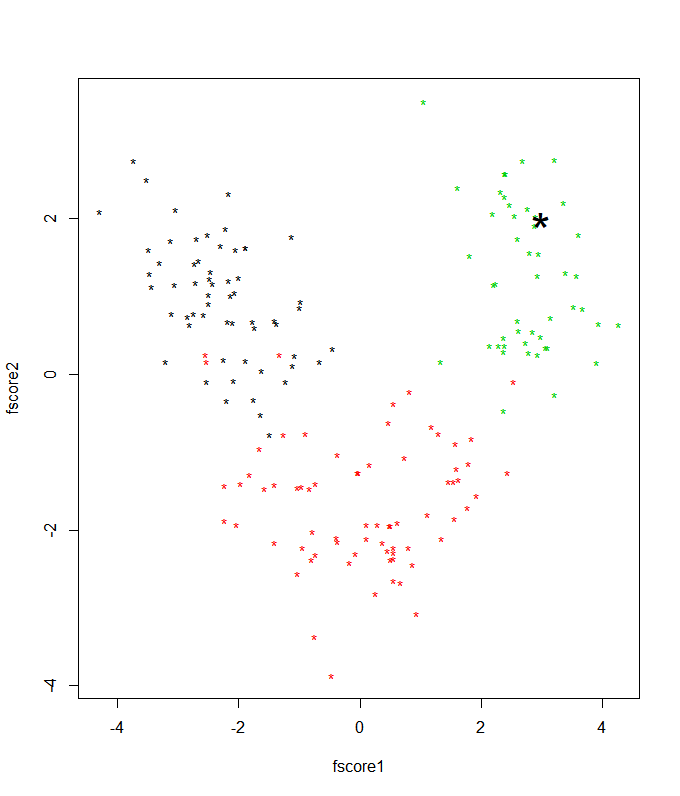
\includegraphics[height=10cm,width=0.9\textwidth]{Rplot.png}
				 \caption{Classificação da nova amostra}
				 \label{fig:fig1}
				 \end{figure}
			 	\end{itemize}
	\end{enumerate}
\end{document}